\documentclass[../main.tex]{subfiles}

\begin{document}
The first of our goals has been extensively addressed in previous
works ~\cite{Bittau08, Krohn2004} through use of the principle of
least privilege. The principle of least privilege (PoLP) requires that
components of a system operate with the minimum resources required to
complete their respective tasks. PoLP is heavily utilized in systems
security research to design systems that maintain their integrity in
the face of an adversary capable of exploiting some of their
components. In contrast, the most popular web servers today execute as
monolithic applications, including Apache and NGINX, where all of
their processes have the same level of privilege and access to the
sensitive key material. Exploiting any one of these processes may
therefore lead to leaking the private key.

To motivate the design of our system, we begin by discussing a system
called Wedge~\cite{Bittau08} that was used to refactor Apache, by
enforcing PoLP, securing the private key in the face of an adversary
who is capable of exploiting the web server application. Wedge's
authors concentrated their efforts on SSL/TLS ciphers that do not
offer forward secrecy, and the scenario where only the client verifies
the server's identity as part of the SSL/TLS handshake.
Figure~\ref{fig:pristrsashake} illustrates the resulting SSL/TLS
handshake. We refer to this handshake as the ``RSA'' handshake for
brevity\footnote{The cipher normally usually used in this handshake is
  RSA; hence the name}. The asymmetric key exchange step is not
necessary here, as mentioned in the previous section. The symmetric
key negotiation step comprises of the client generating a random value
for \texttt{PremasterSecret}, encrypting it in the server's public
key, and sending the resulting packet to the server. Observe that the
long-term private key, as a result, is only used in decrypting
\premaster.

\begin{figure}[H]
  \centering
  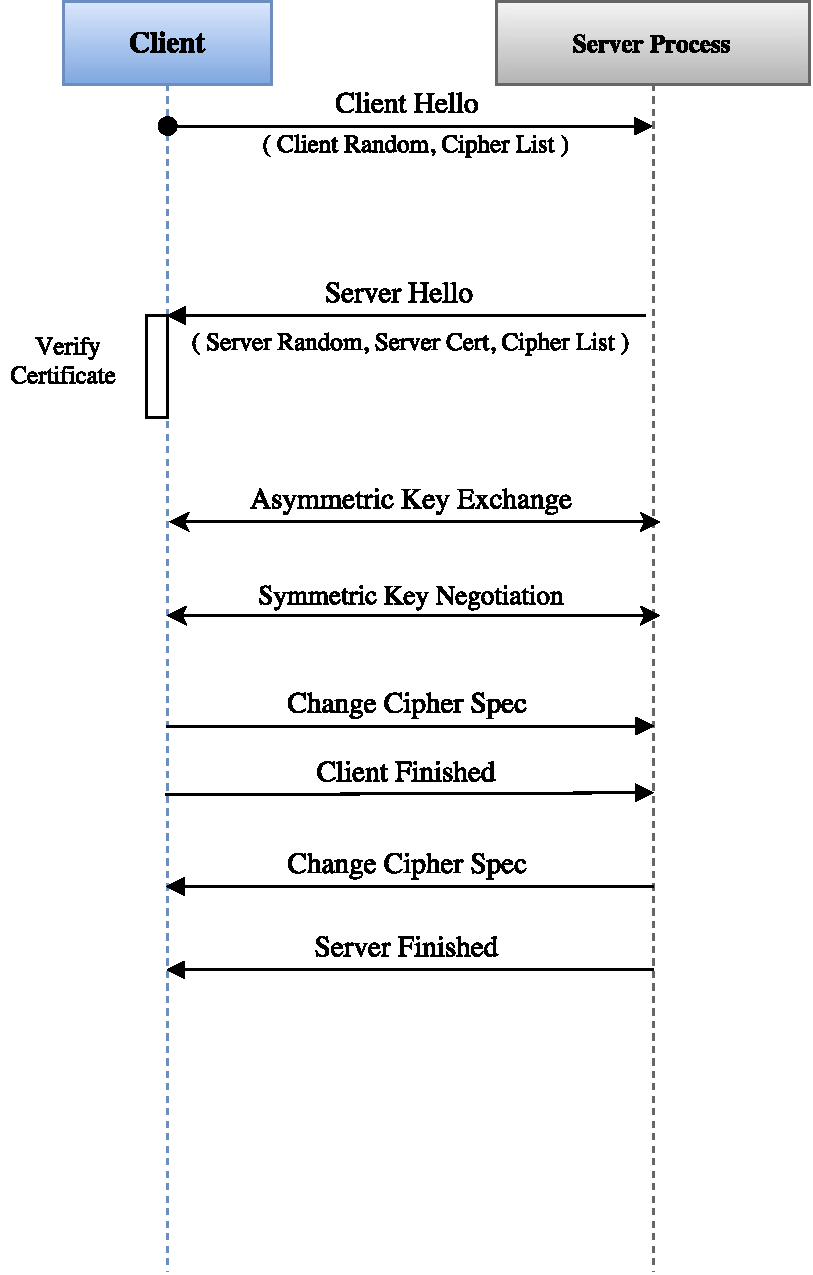
\includegraphics[draft,scale=0.4]{images/rsa-handshake-pristine.pdf}
  \caption[SSL/TLS ``RSA'' handshake]{SSL/TLS handshake for ciphers
    that do not offer forward secrecy. $K$ here is the server's public
    key, and the braces around \texttt{PremasterSecret} indicate the
    packet is encrypted}
  \label{fig:pristrsashake}
\end{figure}

Moving forward, we list the attacks possible against a monolithic web
server, and then detail how the design implemented with Wedge resolved
these vulnerabilities. In this section, we only consider a threat
model where the adversary is capable of passively eavesdropping on
secure communication channels, and exploiting unprivileged components
of the server. We did not consider the second threat model detailed in
the Wedge paper, wherein an attacker is capable of actively modifying
packets exchanged between the web server and client, because the
solution presented in there does not hold if we remove the assumption
that the OS and cloud provider are trusted. This is a consequence of
the web server's user-level processes (dynamic content generation
scripts, databases \&c.)  requiring data in plain-text to complete
their tasks. As such, even if we secure the encrypt/decrypt interface
using the solution in the Wedge paper, plain-text data would
be available in a non-privileged process's memory. This is further
discussed in Section~\ref{sec:design}.

\subsubsection*{Possible Attacks}

There are two main attacks that may be mounted by an adversary capable
of exploiting \textit{only} unprivileged components of the web
server application and passively eavesdropping on packets exchanged
between the server and the client:
 
\begin{enumerate}
  \item The adversary could leak the private key from the network
    facing worker process. This could be done by reading the private key
    from disk directly or from the process's memory space. The attack is
    illustrated in Figure~\ref{fig:attack1}.

    \begin{figure}[H] \centering
      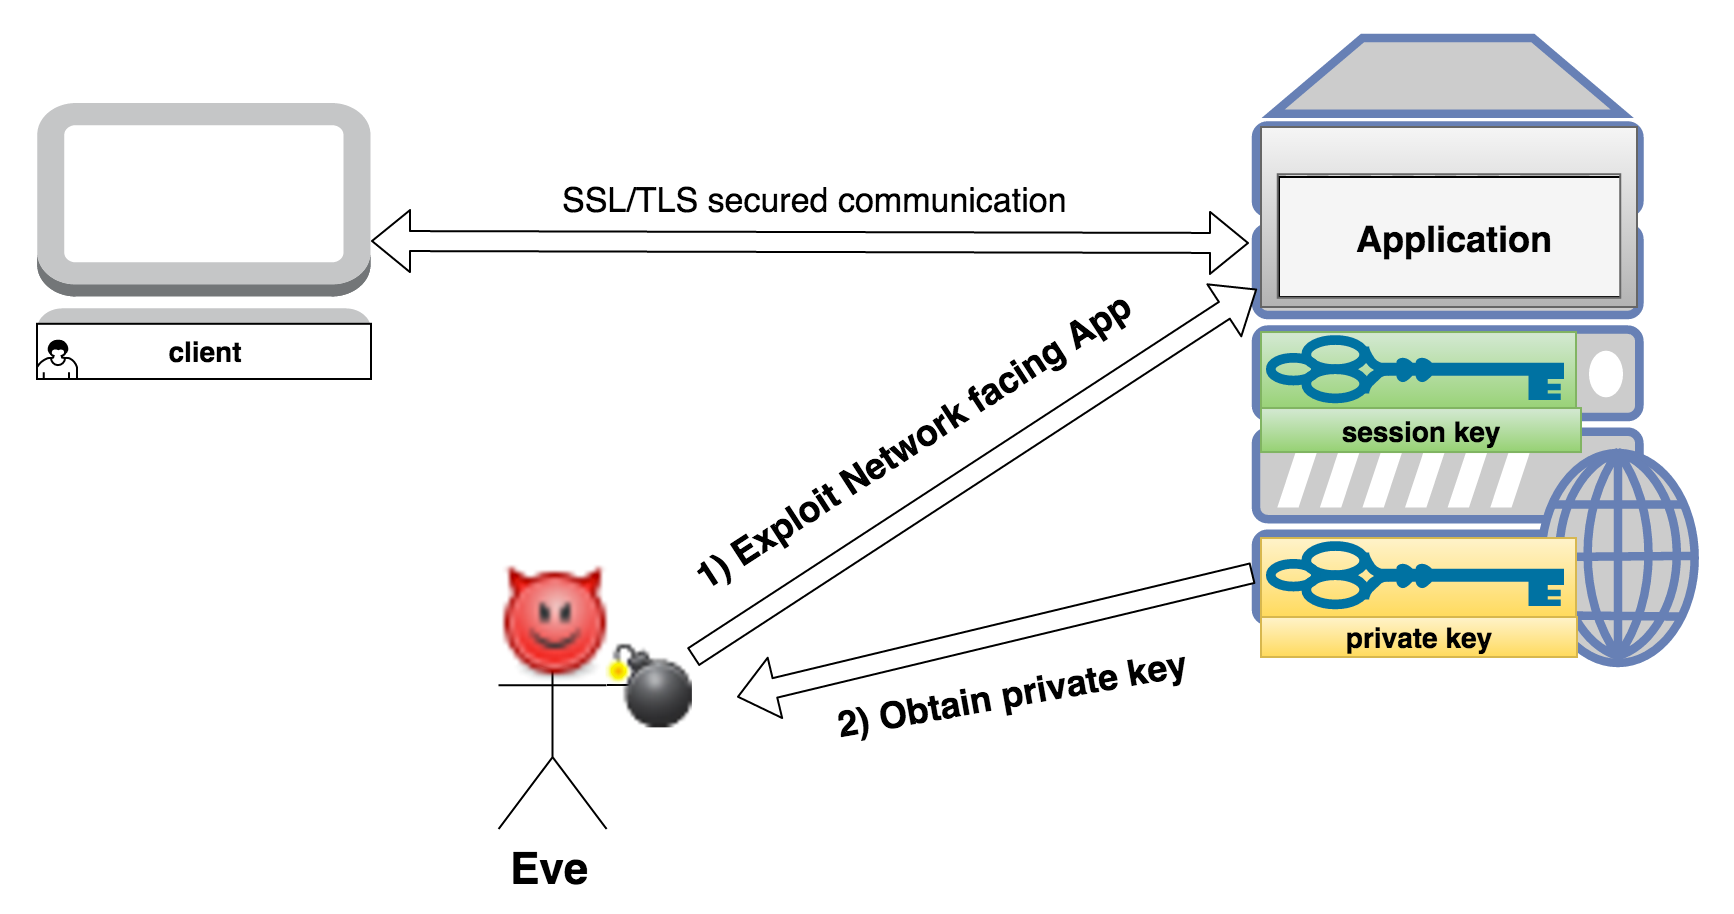
\includegraphics[scale=0.15]{images/attack1.png}
      \caption{Exploiting the network facing component to leak the
        private key}
      \label{fig:attack1}
    \end{figure}

  \item The adversary may record traffic exchanged over the SSL/TLS
    channel and then exploit a naive session key generation interface to
    acquire the session keys used in that exchange. A naive interface is
    one that accepts \crandom, \srandom, and \premaster~ where $K$ is the
    web server's public key.  Such an interface allows an adversary, after
    exploiting the unprivileged component, to generate any previously
    eavesdropped session's symmetric key and is, therefore, no different
    to having read access to the private key from the adversary's
    perspective. This exploit only works if the cipher used is one that
    does not offer forward secrecy, and it only affects the single session
    which was eavesdropped. The attack is illustrated in
    Figure~\ref{fig:attack2}.

    \begin{figure}[H] \centering
      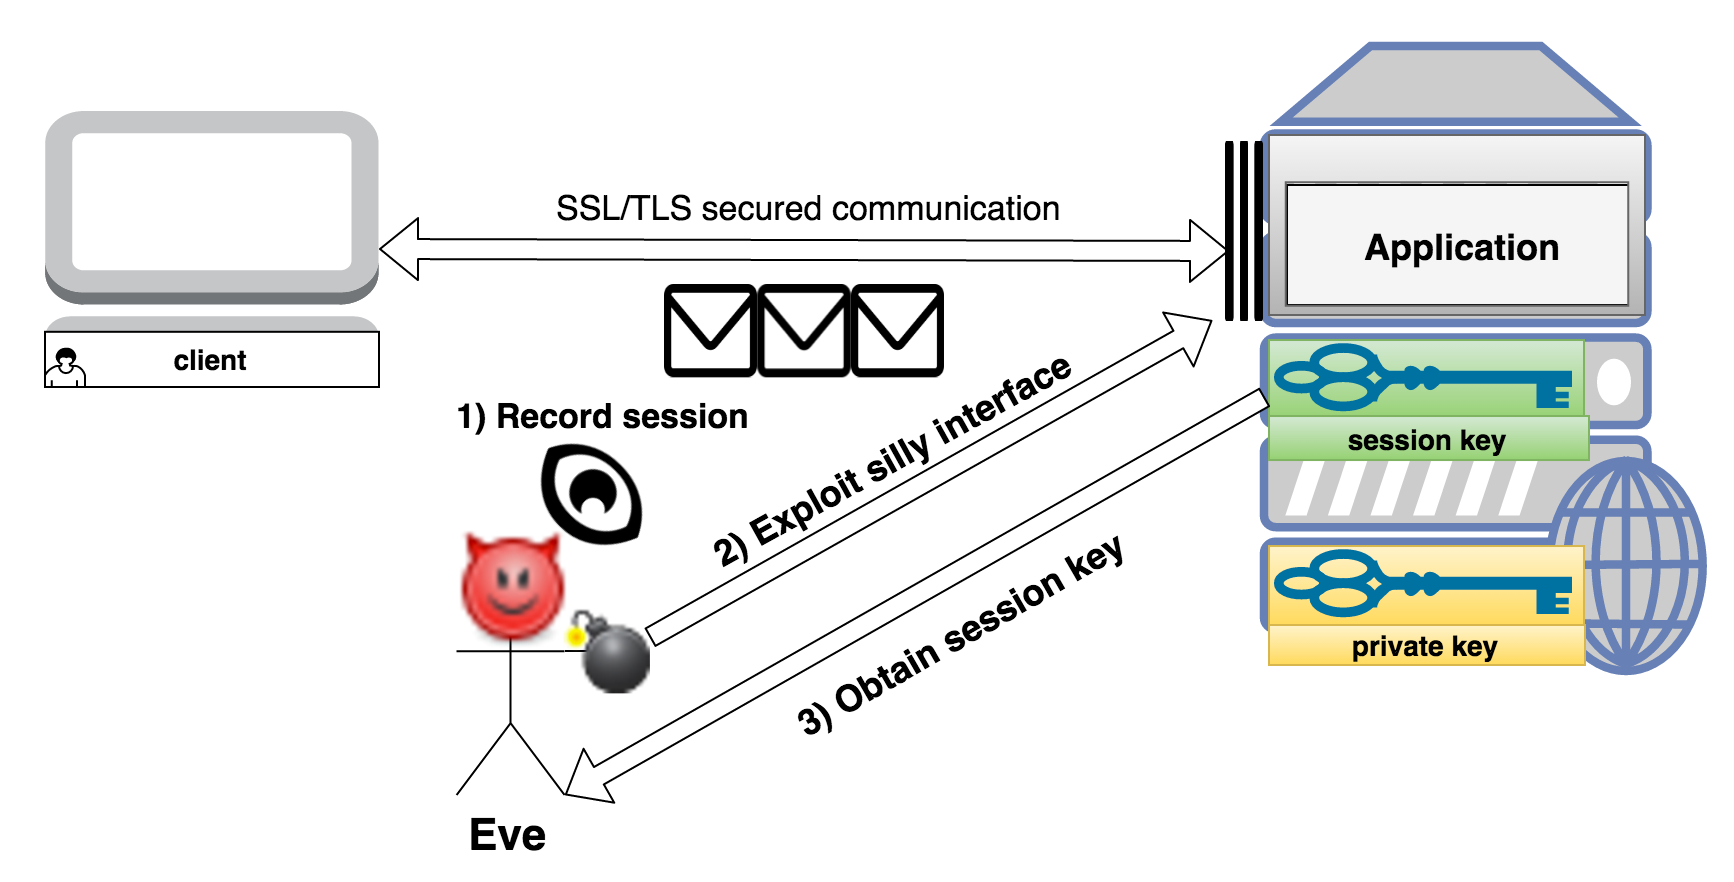
\includegraphics[scale=0.15]{images/attack2.png}
      \caption{Exploiting the network facing component and the naive
        session key generation interface to generate session keys for
        eavesdropped session}
      \label{fig:attack2}
    \end{figure}
\end{enumerate}

\subsubsection*{Proposed Solution}

The solution proposed in the Wedge paper is achieved through
partitioning the session key generation code into its own logical
compartment \footnote{This compartment is called an sthread in Wedge's
  nomenclature} that executes at high privilege. This partitioning can
be seen in Figure~\ref{fig:wedge-partition}.

\begin{figure}[H]
  \centering
  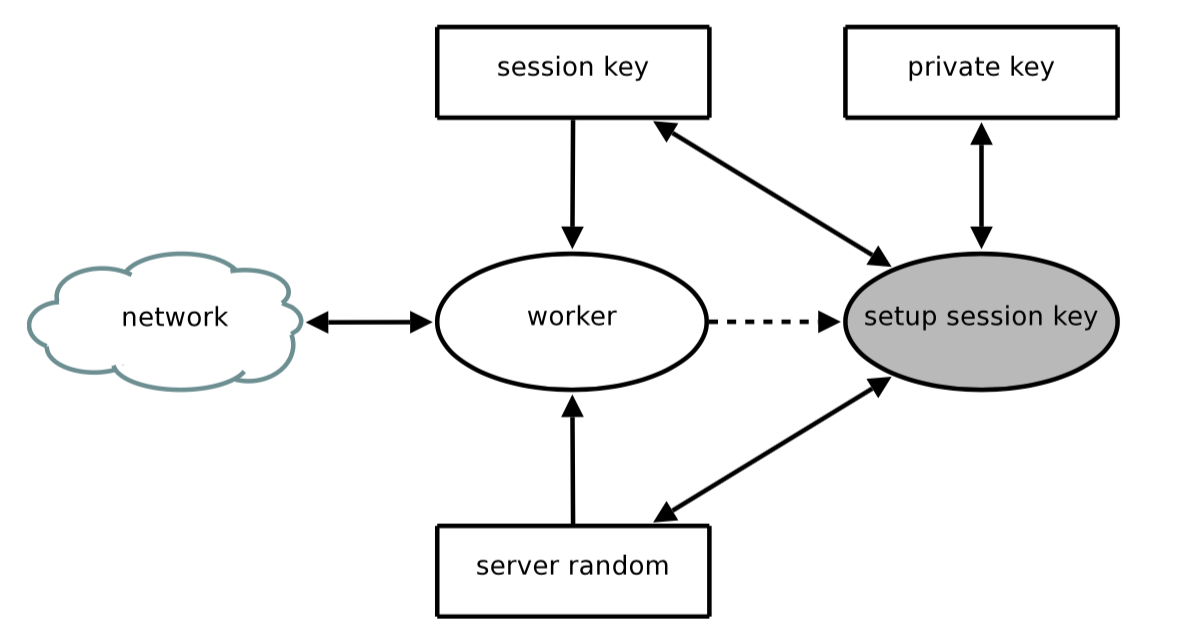
\includegraphics[scale=0.25]{images/compartment_01.png}
  \caption{Partitioning Scheme to protect against leaking the private
    key~\cite{Bittau08}}
  \label{fig:wedge-partition}
\end{figure}

The low privilege worker process does not possess the private key, but
must rely on an interface to the session key generation process. The
interface takes \crandom~ and \premaster~ as arguments, both of which
are provided by the client, while the high privilege component
generates a fresh \srandom~ upon invoking the interface. The freshness
property ensures that, even if an adversary exploits the worker
process, previous session keys cannot be generated by simply invoking
the session key generation interface.

While this design secures the private key against the previously
described adversary, it is not, by itself, sufficient to secure the
key against an adversary capable of exploiting the OS, or from a
malicious cloud-provider with full access to the physical
machine. Such adversaries may leak the key from the privileged
component's memory space by exploiting the OS, or, in the case of the
malicious cloud provider, simply read the key from disk\footnote{Even
b  if the key is encrypted on disk, the decryption key must be present
  in the plain-text binary file for the privileged component, or in
  the process's memory, at runtime, in plain-text}.  A hardware
component, called a trusted platform module, has been utilised in an
effort to secure the private key against the adversaries described
above.

\end{document}
